\chapter{Analysis}

In this chapter, I will present and analyze the data made available by the MCP in the three documents \ttt{E2 - NW-NM DMA Service Instance}, \ttt{E2 - NW-NM REST Service Technical Design}, and \ttt{E2 - NW-NM Service Specification}, which represent all data, made available to me. Furthermore, I will explain the necessity of testing the MCP, as well as present a description of a favorable model structure and potential methods of generating said models.

\section{Data}

To provide a holistic description of a service instance, three documents are necessarily provided. Below are the descriptions of the documents with the service instance \ttt{E2 - NW-NM DMA} as an example.
\begin{description}
  \item[E2 - NW-NM DMA Service Instance]\ \\
    The purpose of this service instance document and its xml-defined counterpart is to describe a DMA instance of the REST-based technical design of the MW- NM service specification, according to the guidelines given in the Service Description Guidelines.
  \item[E2 - NW-NM REST Service Technical Design]\ \\
    The purpose of this service technical design document and its xml-defined counterpart is to describe a REST-based technical design of the MW-NM service specification, according to the guidelines given in the Service Description Guidelines.
  \item[E2 - NW-NM Service Specification]\ \\
    The purpose of this service specification document and its xml-defined counterpart is to provide a holistic overview of the MW-NM service and its building blocks in a technology-independent way, according to the guidelines given in the Service Description Guidelines.
\end{description}
Of the three documents, only the last, \ttt{Service Specification} is to be used to describe specifications of the service, and as such only this will be studied closer.
\section{Service Specification grammar}
The service specification document is constructed using a general xml-format. The majority of the parser grammar of the document can be seen in Figure~\ref{fig:sSpecFull} as well as in Figure~\ref{fig:sSpecRed}, while the latter is in a severely reduced and generalized form. A minority of the grammar has been cut from Figure~\ref{fig:sSpecFull} as it was deemed irrelevant, however the parser grammar in its entirety can be seen in appendices,~\ref{fig:sSpecFull1} and~\ref{fig:sSpecFull2}.

\begin{figure}
  \centering
  \begin{lstlisting}[keywordstyle={}]
ServiceSpecificationSchema ::= specifications

specifications ::= spec specifications
    | $\e$
     
spec ::= name
    | status
    | ID
    | version
    | description
    | keywords
    | isSpatialExclusive
    | authorInfos
    | requirements
    | serviceDataModel
    | serviceInterfaces
     
authorInfos ::= authorInfo authorInfos
    | $\e$

authorInfo ::= aSpec authorInfo
    | $\e$

aSpec ::= ID
    | name
    | description
    | contactInfo

requirements ::= requirement requirements
    | $\e$

requirement ::= rSpec requirement
    | $\e$

rSpec ::= ID
    | name
    | text

serviceDataModel ::= definitionAsXSD

serviceInterfaces ::= serviceInterface serviceInterfaces
    | $\e$

oSpec ::= name
    | description
    | returnValueType
    | parameterTypes
  \end{lstlisting}
  \caption{Snippets of full parser grammar of Service Specification Schema. (Found in appendices~\ref{fig:sSpecFull1}, and~\ref{fig:sSpecFull2})}
  \label{fig:sSpecFull}
\end{figure}

\begin{figure}
  \centering
  \begin{lstlisting}[keywordstyle={}]
ServiceSpecificationSchema ::= specifications

specifications ::= spec specifications
    | $\e$
     
spec ::= specifications
    | spec
    | $\e$

spec ::= string
  \end{lstlisting}
  \caption{Reduced parser grammar of Service Specification Schema.}
  \label{fig:sSpecRed}
\end{figure}

As mentioned above, the service specification is to be used to verify the behavior of the maritime service from a technical stand point. At the moment, the xml-document provides a technical description of its corresponding maritime service, but the most commonly used expression method is free text. As this is a very non-technical design choice, a large portion of the obvious technical advantages provided by the xml-format, is lost. 

As it is possible to utilize free text though the use of natural language processing~\cite{nlp}, no modifications are strictly necessary, however, even with utilization of such or similar methods, implementation hereof would be unstable in terms of usability. This is due to the fact that free language formulation varies at an unforeseeable degree, and as such creating uniform models based on this would add a great layer of complexity.

For a more sustainable solution to the problem, see Section~\ref{sec:Updated Data}.

The xml-version of the service specification can be found in Appendix~\ref{sec:E2 - NW-NM Service Specification}.

\section{Testing the MCP}

The core principle in the MCP is to restructure and streamline maritime software sharing in a manner that can be done the world over, and the very nature of this statement dictates that the platform must be highly scalable. This adds the necessity of running quality-checks on all of the maritime services that are uploaded to the platform. To accommodate this issue, model-based testing immediately seems like the obvious solution, as this technique covers most of the required desired functionality. If implemented satisfyingly, a model-based testing suite for the MCP would be able to:
\begin{enumerate}
  \item Present or verify behavior of maritime services.\\
    There are many obvious common behavioral traits of maritime services, such as adding ships and maritime stakeholders, as well as removing them, however other behavioral patterns will often vary to the point of lowered manageability. A model, describing the maritime service in question will provide a clear and undeniable description of the service's behavior.\newpage
  \item Visualize functionality of maritime services.\\
    Just as well as behavioral traits, functionality will differ greatly from one maritime service to another, and therefore it is very useful for a model to visualize said functionality, as well as verifying that it works as intended.
  \item Present the structures of maritime services.\\
    This trait will be used to visualize the structural components of maritime services. Just as point one and two, this functionality will be useful for creating a quick and clear projection of how the maritime service behaves.
  \item Increase reliability and efficiency of maritime services.\\
    Through correct implementation of points one, two, and three, it is possible to elevate the reliability and efficiency of the maritime services, found on the MCP. This is due to the same reasoning that all testing is conducted on the basis of: the need for safe, consistent, and correct code.
\end{enumerate}
\noindent
As stated in Section~\ref{sec:Model-Based Testing} there are two main types of model-based testing techniques: serial and sequential model building-and testing, and as these two techniques both provide different advantages utilizing either one will be a trade-off.\newpage

\section{Example Model Structure}
Throughout this report, I will use a map-requesting service as an example. In this example the maritime service will act as an intermediate, broking between a ship and a company, where the map is being held. The ship will have to submit authentication information to the maritime service in order to get a the requested map. The model, which has been built upon the example protocol has been illustrated in Figure~\ref{fig:modelExProtocol}. The lines numbered 1-6 illustrate interaction between the three entities \ttt{Ship}, \ttt{Service}, and \ttt{Company}, where *1 and *2 respectively, illustrate a submitting of authentication information to the service, and the service accepts the information and sends a response. *3 and *4 illustrates the service's request of the requested map, and its subsequent receiving hereof. *5 illustrates the forwarding of requested information to the ship.
\begin{figure}[h!]
  \centering
  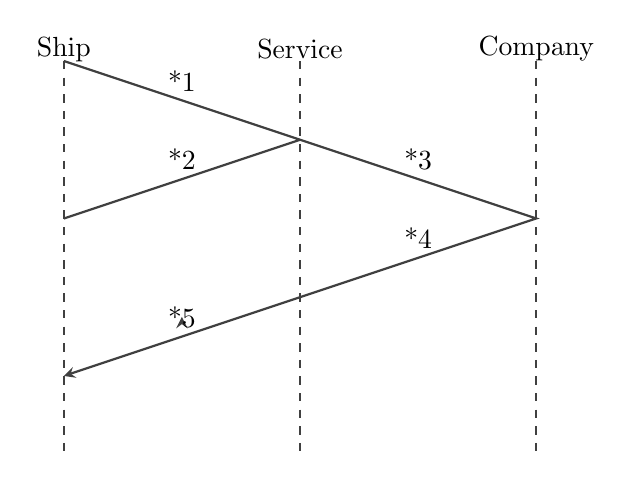
\begin{tikzpicture}[thick]
    % timelines
    \draw [dashed]  (0,5) --  (0,0)
          [dashed]  (3,5) --  (3,0)
          [dashed]  (6,5) --  (6,0)
    
    % entity labels
          (0,5.15)  node  {Ship}
          (3,5.15)  node  {Service}
          (6,5.15)  node  {Company}

    % interaction labels
          (1.5,4.75)  node  {*1}
          (1.5,3.75)  node  {*2}
          (4.5,3.75)  node  {*3}
          (4.5,2.75)  node  {*4}
          (1.5,1.75)  node  {*5};
    % interaction lines
    \draw (0,5) --  (3,4) --  (0,3)  % API call (request/response)
          (3,4) --  (6,3) --  (0,1); % Service requests/recieves data from company/data center and Information is forwarded to the ship.
  \end{tikzpicture}
  \caption{Early draft of a model example, where a ship requests information from a service.}
  \label{fig:modelExProtocol}
\end{figure}
Figure~\ref{fig:fsmExShip} represents an FSM, illustrating the \ttt{ship} entity in Figure~\ref{fig:modelExProtocol}. The FSM starts in the \ttt{No map loaded} state, and has the three available actions, \ttt{trash map}, \ttt{request map}, and \ttt{await response}. Performing \ttt{trash map} or \ttt{await response} in the initial state will yield no results, as no map is available to be trashed and no response is on the way. If \ttt{request map} is performed, the state will be changed to the intermediate state \ttt{awaiting map}, where \ttt{await response} is the only action that will change the state, as no map can be trashed, and requesting another map will change the state to the same, but where a different map is being waited for. The third and final state \ttt{map loaded} will allow the actions \ttt{trash map}, which will change the state to \ttt{no map loaded} and \ttt{request map}, which will, respectively, trash the loaded map, and request a new one, changing the state to \ttt{awaiting map}.
\newpage
\noindent
Figure~\ref{fig:fsmExService} represents an FSM, illustrating the \ttt{service} entity in Figure~\ref{fig:modelExProtocol}. The FSM has the two states, \ttt{idle} and \ttt{active}, the former being the initial state. Whenever the entity receives a valid response the state changes to the \ttt{active} state, and when the request has been properly handled, the state changes back to \ttt{idle}.
\begin{figure}[h]
  \centering
  \begin{tikzpicture}[->,>=stealth', node distance=3.5 cm, thick]
    \tikzstyle{every state}=[rectangle,
                       draw=gray,
                       rounded corners,
                       rectangle,
                       top color=white,
                       bottom color=gray!50]
    \tikzstyle{every path}=[->,gray!150,>=stealth,text=black]

    \node[state, initial] (A) []                {No map loaded};
    \node[state]          (B) [below left of=A] {Awaiting Map};
    \node[state]          (C) [below right of=A]{Map loaded};

    \path (A) edge[bend right,left]                                   node{Request Map}   (B)
              edge[loop above,left,       out=130,in=100, looseness=7]node{Trash Map}     (A)
          (B) edge[loop above,below left, out=130,in=100, looseness=7]node{Request Map}   (B)
              edge[loop below,below,      out=240,in=270, looseness=7]node{Trash Map}     (B)
              edge[bend right,below]                                  node{Await Response}(C)
          (C) edge[bend right,above]                                  node{Request Map}   (B)
              edge[bend right,right]                                  node{Trash Map}     (A);
  \end{tikzpicture}
  \caption{FSM, describing the \ttt{Ship} entity in Figure~\ref{fig:modelExProtocol}.}
  \label{fig:fsmExShip}
\end{figure}
\begin{figure}[h]
  \centering
  \begin{tikzpicture}[->,>=stealth', node distance=3.5 cm, thick]
    \tikzstyle{every state}=[rectangle,
                       draw=gray,
                       rounded corners,
                       rectangle,
                       top color=white,
                       bottom color=gray!50]
    \tikzstyle{every path}=[->,gray!150,>=stealth,text=black]
    \node[state, initial] (A) []      {Idle};
    \node[state]      (B) [right of=A]{Active};

    \path (A) edge[loop above,left,  align=center, out=130,in=100, looseness=7]node{Process Request\\(Invalid Request)}(A)
              edge[bend left, above, align=center]                             node{Process Request\\(Valid Request)}  (B)
          (B) edge[bend left, below]                                           node{Respond}                           (A);
  \end{tikzpicture}
  \caption{FSM, describing the \ttt{Service} entity in Figure~\ref{fig:modelExProtocol}.}
  \label{fig:fsmExService}
\end{figure}

\section{Uses of model-based testing of the MCP}
The main advantage that comes from model-based testing is the large variety in testing algorithms it produces. If a model is to be machine readable the techniques, listed below can be implemented fully automatic, and if not, they can still be utilized manually. The following techniques can be applied to true and fair maritime service-models in the MCP: \newpage
\begin{description}
  \item[Finite state machines]\ \\
    As mentioned in Section~\ref{ssec:Finite State Machines (FSM)}, a FSM is made up of states, and the ability of a simulating program to change state through a collection of actions. Executable paths are determined, which can be used to create test cases, as well as illustrate the behavior of the system. Furthermore FSMs are closely related to the further techniques, that will be explained below.
  \item[Proving theorems]\ \\
    Automatic theorem proving is a technique originally produced for proving logical formulas, which is a concept that can be rewritten to suit model-based testing. In order to create test cases, system behavior is assigned to equivalence classes. Following this step, predicates can be formed from equivalence classes and logical consequences of the equivalence classes. 
  \item[Symbolic execution]\ \\
    Much in the likes of an FSM, a symbolic execution of a program or system will generate executable paths, along with symbolic values, describing how they can be accessed. A symbolic execution engine will analyze possible variations of input in order to create a map of the software in question. Said map can subsequently be used to better understand, test, and develop the software in question.
  \item[Model checkers]\ \\
    Model checkers, also known as property checkers, are methods of determining if an FSM meets a specific set of requirements. The model checkers detect if requirements are met, either by determining examples or counterexamples. When a path, representing either an example or a counterexample is discovered it is logged as a \tit{witness}, which can be mutated upon when generating test cases.
  \item[Markov chains]\ \\
    Markov chains are named after the Russian mathematician Andrew Markov, and are also known as usage models. A Markov chain, or usage model, is made up of two primary components; firstly an FSM, which represents every available action of a given system, and secondly an operational profile, which is a statistical indicator of what has been or will be used. The FSM is used by the operational profile in order to generate the statistical analysis, and the operational profile is used by the FSM to derive operational tests.
\end{description}
The scope of which features the above techniques will be able to test, will be deemed by the actual maritime service model, however, the expansive array of methods will cover maritime services extensively.
\section{Use-Cases}
In this section, I will present the utilization of the desired tool, that is implemented throughout Chapter~\ref{chp:Work/Design} using techniques described in Chapter~\ref{chp:Analysis}. This entails three examples, described in Figures~\ref{fig:useCaseVerifyFirst} through~\ref{fig:useCaseIncorrect}, and visualized in Figure~\ref{fig:useCaseDiagram}. Figures~\ref{fig:useCaseVerifyFirst} and~\ref{fig:useCaseVerifySecond} describe intended use of the implementation, while Figure~\ref{fig:useCaseIncorrect} describes unintended use of the implementation. Actor/system-interaction is described in Figure~\ref{fig:useCaseDiagram}.
\begin{figure}[h]
  \centering
  \begin{tabular}{l|l} \toprule
    Use Case   & System verifies model, first iteration \\ \midrule
    Actors     & Service Instance Designer (SD) \\ \midrule
    Basic Flow & \makecell[l]{1. SD will submit a service specification.\\
                              2. SD submits all information as per the old service\\
                              \ \ \ \ specification syntax.\\
                              3. SD submits all information to generate maritime model. \\
                              4. Model concept is tested and accepted. \\
                              5. SD submits the service instance specification.}  \\ \bottomrule
  \end{tabular}
  \caption{First example of correct use of the solution.}
  \label{fig:useCaseVerifyFirst}
\end{figure}
\begin{figure}[h]
  \centering
  \begin{tabular}{l|l} \toprule
    Use Case   & System verifies model, second iteration \\ \midrule
    Actors     & Service Instance Designer (SD) \\ \midrule
    Basic Flow & \makecell[l]{1. SD will submit a service specification.\\
                              2. SD submits all information as per the old service\\
                              \ \ \ \ specification syntax.\\
                              3. SD submits all information to generate maritime model. \\
                              4. Model concept is tested and rejected.\\
                              5. SD repeats step 3.\\
                              6. Model concept is tested and verified. \\
                              7. SD submits the service instance specification.}  \\ \bottomrule
  \end{tabular}
  \caption{Second example of correct use of the solution.}
  \label{fig:useCaseVerifySecond}
\end{figure}
The steps described in Figures~\ref{fig:useCaseVerifyFirst} and~\ref{fig:useCaseVerifySecond} are similar up until 4, where one example accepts, while the other example rejects the model. As the Service Instance Designer produces a valid model in Figure~\ref{fig:useCaseVerifyFirst}, the fact that the system is used correctly is trivial, and while the initial model is rejected, based on the desired behavior in Figure~\ref{fig:useCaseVerifySecond}, the final result is a valid model concept, and thus the software has been used as intended.
\newpage
\noindent
In the case of Figure~\ref{fig:useCaseIncorrect} a model is created, using the system, similar to above, however, the result of the checked input is ignored by the user. This should still be possible, as the limitations of the system, should not be projected onto the created software, but in some instances, it could also lead to invalid model-concepts being iterated upon further.
\begin{figure}[h]
  \centering
  \begin{tabular}{l|l} \toprule
    Use Case   & User ignores model warnings \\ \midrule
    Actors     & Service Instance Designer (SD) \\ \midrule
    Basic Flow & \makecell[l]{1. SD will submit a service specification.\\
                              2. SD submits all information as per the old service\\
                              \ \ \ \ specification syntax.\\
                              3. SD submits all information to generate maritime model. \\
                              4. Model concept is tested and rejected.\\
                              5. SD submits the service instance specification.}  \\ \bottomrule
  \end{tabular}
  \caption{Incorrect use of the solution.}
  \label{fig:useCaseIncorrect}
\end{figure}
\begin{figure}
  \centering
  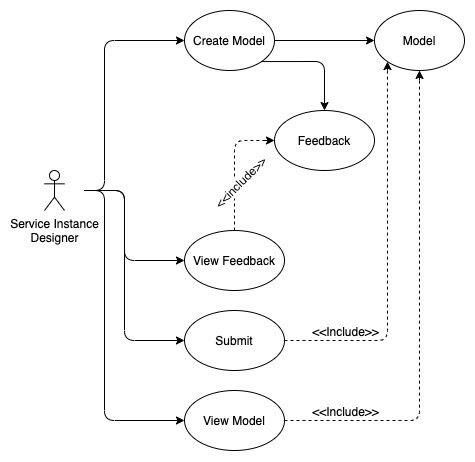
\includegraphics[width=0.8\linewidth]{figures/UCD.jpg}
  \caption{Use case diagram describing Figures~\ref{fig:useCaseVerifyFirst},~\ref{fig:useCaseVerifySecond}, and~\ref{fig:useCaseIncorrect}.}
  \label{fig:useCaseDiagram}
\end{figure}
\newpage
\section{Summary: Advantages and Disadvantages} 
Issues will inevitably present themselves with a project such as this, however the scope and nature of these issues will vary with each approach possible. As different approaches offer tailored advantages to circumvent correlating unique concerns, another set of unique concerns will necessarily present themselves. In this section I will sum up the approaches presented throughout Chapter~\ref{chp:Analysis}, along with their corresponding arising advantages and disadvantages.
\subsection{Manual model-creation}
\tbf{Advantages}
\begin{itemize}
  \item Manual model creation will have a shorter initial implementation time, as an arbitrary single model is faster to build than its auto-model-generator counterpart. 
  \item Built maritime service models can be fully customized at once in order to describe all aspects of its maritime service counterparts.
  \item Having customized each maritime service model to its corresponding maritime service counterpart allows for an equally customized test suite. Following this, the techniques, described in Section~\ref{sec:Uses of model-based testing of the MCP}, will allow for exhaustive tests via manual model-creating.
\end{itemize}
\tbf{Disadvantages}
\begin{itemize}
  \item The time consumption of manually creating each model will expand near-linearly with each maritime service, that is submitted, and subsequently needs a maritime service model. 
  \item Having each maritime service model being created individually and manually will inevitably introduce much diversity both in the sense of the available standard actions and implementation style of the model.
  \item The complexity as well as way of implementing testing techniques explained in Section~\ref{sec:Uses of model-based testing of the MCP} varies to an extent, even without consideration of non-uniform models. Elaborating on the case that each maritime service model differs both in purpose, implementation style and exhaustiveness, creating test suites similar to those described in Section~\ref{sec:Uses of model-based testing of the MCP} for each new maritime service, will become an extensive project.
\end{itemize}\newpage
\subsection{Automatic model-creation}
\tbf{Advantages}
\begin{itemize}
  \item The first and foremost advantage of automatic model generation is the scalability it provides. This comes as the implementation of \tit{one} maritime service model generator module, ideally, will be able to automatically assemble each maritime model without further interference, as opposed to manual model generating.
  \item As an automatic model generator abides by a set collection of rules and metrics, and would create models following the instructions of an xml specification-file, generated models will never deviate from the uniformity of the generator.
  \item The uniformity in the generated models will further show advantage, as this will streamline test suite generation either because of the fact that similar models promote similar manual test suite generation, or because that it allows for near-total automation.
\end{itemize}
\tbf{Disadvantages}
\begin{itemize}
  \item The obvious disadvantage that comes with automatic model generation, is the lack of customization in models. As the generator should handle all models that can be described through the xml specification files, it needs to be generalized, which in turn means less specific models, which lowers the ability to custom-fit each model to its maritime specification counterpart.
  \item Another inevitable downside of having automatically generated - however less specific - models is the fact that test suites can become less specific, and in extension hereof less exhaustive of the maritime service.
\end{itemize}
\indent
To sum up, both methods will be advantageous, as they will each allow for extensive testing, with the former being more custom-tailored and so a lot more time consuming in the long run, and the latter being more generic, but much ultimately less time consuming in the long run.